\rfcnumber{0008}
\rfctitle{Session Data Protocol}
\rfcdate{October 2025}
\rfcauthor{Tino Breddin (@tolbrino), Lukas Pohanka (@NumberFour8)}
\section{RFC-0008: Session Data
Protocol}\label{rfc-0008-session-data-protocol}

\begin{itemize}
\tightlist
\item
  \textbf{RFC Number:} 0008
\item
  \textbf{Title:} Session Data Protocol
\item
  \textbf{Status:} Finalised
\item
  \textbf{Author(s):} Tino Breddin (@tolbrino), Lukas Pohanka
  (@NumberFour8)
\item
  \textbf{Created:} 2025-08-15
\item
  \textbf{Updated:} 2025-10-27
\item
  \textbf{Version:} v1.0.0 (Finalised)
\item
  \textbf{Supersedes:} none
\item
  \textbf{Related Links:}
  \href{../RFC-0002-mixnet-keywords/0002-mixnet-keywords.md}{RFC-0002},
  \href{../RFC-0004-hopr-packet-protocol/0004-hopr-packet-protocol.md}{RFC-0004},
  \href{../RFC-0009-session-start-protocol/0009-session-start-protocol.md}{RFC-0009}
\end{itemize}

\subsection{1. Abstract}\label{abstract}

This RFC specifies the HOPR session data protocol, which provides
reliable and unreliable data transmission capabilities over the HOPR
mixnet. The protocol implements TCP-like features {[}01{]} including
message segmentation, reassembly, acknowledgement, and retransmission,
whilst maintaining simplicity and efficiency suitable for mixnet
deployment. This protocol works in conjunction with the HOPR session
start protocol
(\href{../RFC-0009-session-start-protocol/0009-session-start-protocol.md}{RFC-0009})
to provide complete session management capabilities for applications
within the HOPR ecosystem.

The protocol supports both reliable (TCP-like) and unreliable (UDP-like)
transmission modes, allowing applications to choose the appropriate
trade-off between reliability and latency for their use case.

\subsection{2. Motivation}\label{motivation}

The HOPR mixnet uses HOPR packets
(\href{../RFC-0004-hopr-packet-protocol/0004-hopr-packet-protocol.md}{RFC-0004})
to transport data between nodes. This fundamental packet-sending
mechanism operates as a fire-and-forget transport similar to UDP
{[}03{]}, providing no guarantees of delivery, ordering, or message
boundaries. Whilst this simplicity is appropriate for the packet layer,
application developers typically require higher-level features such as:

\begin{itemize}
\tightlist
\item
  \textbf{Reliable delivery}: ensuring that messages are delivered or
  that the sender is notified of failures
\item
  \textbf{Message ordering}: receiving messages in the order they were
  sent
\item
  \textbf{Message segmentation}: handling messages larger than the fixed
  packet size
\item
  \textbf{Flow control}: managing transmission rates to prevent
  overwhelming receivers
\end{itemize}

To ease adoption, HOPR nodes must provide a way for applications to use
these features without reimplementing TCP {[}01{]} or UDP {[}02{]} from
scratch. Since the HOPR protocol is not IP-based, implementing these
protocols directly would require complex IP protocol emulation.

The HOPR session data protocol fills this gap by providing both reliable
and unreliable data transmission modes directly over the HOPR packet
transport. Session establishment and lifecycle management are handled by
the HOPR session start protocol
(\href{../RFC-0009-session-start-protocol/0009-session-start-protocol.md}{RFC-0009}),
whilst this protocol focuses exclusively on efficient data transmission
once a session is established.

\subsection{3. Terminology}\label{terminology}

The keywords ``MUST'', ``MUST NOT'', ``REQUIRED'', ``SHALL'', ``SHALL
NOT'', ``SHOULD'', ``SHOULD NOT'', ``RECOMMENDED'', ``MAY'', and
``OPTIONAL'' in this document are to be interpreted as described in
{[}03{]} when, and only when, they appear in all capitals, as shown
here.

All terminology used in this document, including general mix network
concepts and HOPR-specific definitions, is provided in
\href{../RFC-0002-mixnet-keywords/0002-mixnet-keywords.md}{RFC-0002}.
That document serves as the authoritative reference for the terminology
and conventions adopted across the HOPR RFC series.

Terms defined in
\href{../RFC-0002-mixnet-keywords/0002-mixnet-keywords.md}{RFC-0002} are
used. Additionally, this document defines the following
session-protocol-specific terms:

\begin{itemize}
\item
  \textbf{frame}: a logical unit of data transmission in the session
  protocol. Frames can be of arbitrary length and are identified by a
  unique frame ID. Frames represent complete application messages that
  may span multiple packets.
\item
  \textbf{segment}: a fixed-size fragment of a frame. Frames larger than
  the packet MTU are split into segments for transmission, with each
  segment carrying metadata about its position within the frame to
  enable reassembly.
\item
  \textbf{frame ID}: a 32-bit unsigned integer that uniquely identifies
  a frame within a session (1-indexed, starting from 1). Frame ID values
  are interpreted as big-endian unsigned integers and increment
  sequentially with each new frame.
\item
  \textbf{sequence number (SeqNum)}: an 8-bit unsigned integer
  indicating a segment's position within its frame (0-indexed, starting
  from 0). This enables correct reassembly of frames from segments.
\item
  \textbf{sequence flags (SeqFlags)}: an 8-bit value encoding additional
  segment metadata, including whether the segment is the final segment
  of a frame and whether it represents a terminating segment.
\item
  \textbf{session socket}: the endpoint abstraction that implements the
  session protocol, available in both reliable and unreliable variants.
  Session sockets provide familiar send/receive APIs to applications.
\item
  \textbf{MTU (maximum transmission unit)}: the maximum size of a single
  HOPR protocol message payload, denoted as \codebubble{C} throughout
  this specification. This is determined by the packet format defined in
  \href{../RFC-0004-hopr-packet-protocol/0004-hopr-packet-protocol.md}{RFC-0004}.
\item
  \textbf{terminating segment}: a special segment with the termination
  flag set that signals the graceful end of a session. Terminating
  segments carry no data payload.
\end{itemize}

\subsection{4. Specification}\label{specification}

\subsubsection{4.1 Protocol Overview}\label{protocol-overview}

The HOPR session data protocol operates at version 1 and consists of
three message types that work together to provide reliable or unreliable
data transmission:

\begin{enumerate}
\def\labelenumi{\arabic{enumi}.}
\tightlist
\item
  \textbf{segment messages}: Carry actual data fragments
\item
  \textbf{retransmission request messages}: Request missing segments
\item
  \textbf{frame acknowledgement messages}: Confirm successful frame
  receipt
\end{enumerate}

The protocol supports two operational modes:

\begin{itemize}
\tightlist
\item
  \textbf{Unreliable Mode}: Fast, stateless operation similar to UDP
  {[}04{]}
\item
  \textbf{Reliable Mode}: Stateful operation with acknowledgements and
  retransmissions
\end{itemize}

Session establishment and lifecycle management are handled by the HOPR
Session Start Protocol. All multi-byte integer fields use network byte
order (big-endian) encoding to ensure consistent interpretation across
different architectures.

\subsubsection{4.2 Session Data Protocol Message
Format}\label{session-data-protocol-message-format}

All Session Data Protocol messages follow a common structure:

\begin{figure}
\centering
\pandocbounded{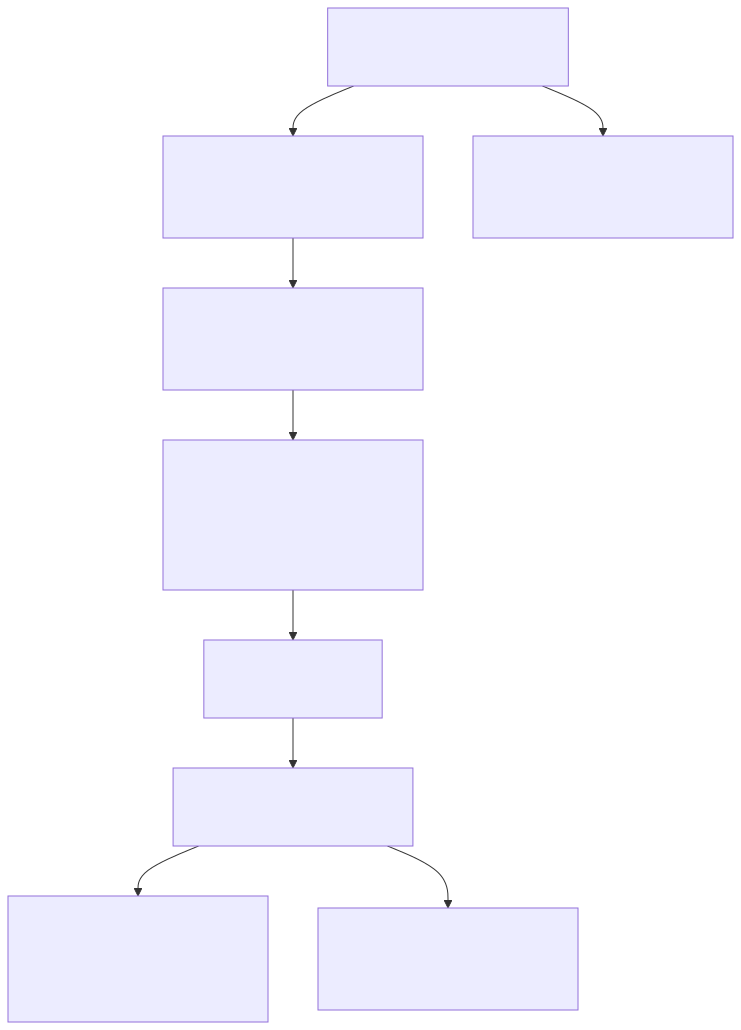
\includegraphics[width=\maxwidth,keepaspectratio,alt={Mermaid Diagram 1}]{0008-session-protocol/mermaid_1.png}}
\caption{Mermaid Diagram 1}
\end{figure}

\begin{longtable}[]{@{}
  >{\raggedright\arraybackslash}p{(\linewidth - 6\tabcolsep) * \real{0.1486}}
  >{\raggedright\arraybackslash}p{(\linewidth - 6\tabcolsep) * \real{0.1081}}
  >{\raggedright\arraybackslash}p{(\linewidth - 6\tabcolsep) * \real{0.3378}}
  >{\raggedright\arraybackslash}p{(\linewidth - 6\tabcolsep) * \real{0.4054}}@{}}
\toprule\noalign{}
\begin{minipage}[b]{\linewidth}\raggedright
Field
\end{minipage} & \begin{minipage}[b]{\linewidth}\raggedright
Size
\end{minipage} & \begin{minipage}[b]{\linewidth}\raggedright
Description
\end{minipage} & \begin{minipage}[b]{\linewidth}\raggedright
Value
\end{minipage} \\
\midrule\noalign{}
\endhead
\bottomrule\noalign{}
\endlastfoot
\textbf{Version} & 1 byte & Protocol version & MUST be \codebubble{0x01}
for version 1 \\
\textbf{Type} & 1 byte & Message type discriminant & See Message Types
table below \\
\textbf{Length} & 2 bytes & Payload length in bytes & Maximum is
\codebubble{C - 4} \\
\textbf{Payload} & Variable & Message-specific data & Format depends on
message type \\
\end{longtable}

\paragraph{4.2.1 Message Types}\label{message-types}

\begin{longtable}[]{@{}
  >{\raggedright\arraybackslash}p{(\linewidth - 4\tabcolsep) * \real{0.1471}}
  >{\raggedright\arraybackslash}p{(\linewidth - 4\tabcolsep) * \real{0.3431}}
  >{\raggedright\arraybackslash}p{(\linewidth - 4\tabcolsep) * \real{0.5098}}@{}}
\toprule\noalign{}
\begin{minipage}[b]{\linewidth}\raggedright
Type Code
\end{minipage} & \begin{minipage}[b]{\linewidth}\raggedright
Name
\end{minipage} & \begin{minipage}[b]{\linewidth}\raggedright
Description
\end{minipage} \\
\midrule\noalign{}
\endhead
\bottomrule\noalign{}
\endlastfoot
\codebubble{0x00} & Segment & Carries actual data fragments \\
\codebubble{0x01} & Retransmission Request & Requests missing
segments \\
\codebubble{0x02} & Frame Acknowledgement & Confirms successful frame
receipt \\
\end{longtable}

\clearpage

\paragraph{4.2.2 Byte Order}\label{byte-order}

All multi-byte integer fields and values in the Session Data Protocol
MUST be encoded and interpreted in network byte order (big-endian). This
applies to:

\textbf{Protocol Message Fields:}

\begin{itemize}
\tightlist
\item
  \textbf{Length} field (2 bytes) in the common message format
\item
  \textbf{Frame ID} field (4 bytes) in Segment, Retransmission Request,
  and Frame Acknowledgement messages
\item
  Any future numeric fields added to the protocol
\end{itemize}

This requirement ensures consistent interpretation across different
architectures and prevents interoperability issues between
implementations.

\subsubsection{4.3 Segment Message}\label{segment-message}

\paragraph{4.3.1 Segment Structure}\label{segment-structure}

\begin{figure}
\centering
\pandocbounded{\includegraphics[width=\maxwidth,keepaspectratio,alt={Mermaid Diagram 2}]{0008-session-protocol/mermaid_2.png}}
\caption{Mermaid Diagram 2}
\end{figure}

\begin{longtable}[]{@{}
  >{\raggedright\arraybackslash}p{(\linewidth - 6\tabcolsep) * \real{0.1979}}
  >{\raggedright\arraybackslash}p{(\linewidth - 6\tabcolsep) * \real{0.0833}}
  >{\raggedright\arraybackslash}p{(\linewidth - 6\tabcolsep) * \real{0.4062}}
  >{\raggedright\arraybackslash}p{(\linewidth - 6\tabcolsep) * \real{0.3125}}@{}}
\toprule\noalign{}
\begin{minipage}[b]{\linewidth}\raggedright
Field
\end{minipage} & \begin{minipage}[b]{\linewidth}\raggedright
Size
\end{minipage} & \begin{minipage}[b]{\linewidth}\raggedright
Description
\end{minipage} & \begin{minipage}[b]{\linewidth}\raggedright
Valid Range
\end{minipage} \\
\midrule\noalign{}
\endhead
\bottomrule\noalign{}
\endlastfoot
\textbf{Frame ID} & 4 bytes & Frame identifier & 1 to 4,294,967,295 \\
\textbf{Sequence Number} & 1 byte & Segment position within frame
(0-based) & 0-63 \\
\textbf{Sequence Flags} & 1 byte & Segment metadata flags & See Sequence
Flags table below \\
\textbf{Segment Data} & Variable & Payload data & 0 to
(\codebubble{C - 10}) bytes \\
\end{longtable}

\clearpage

\paragraph{4.3.2 Sequence Flags Bitmap}\label{sequence-flags-bitmap}

\begin{longtable}[]{@{}
  >{\raggedright\arraybackslash}p{(\linewidth - 6\tabcolsep) * \real{0.0353}}
  >{\raggedright\arraybackslash}p{(\linewidth - 6\tabcolsep) * \real{0.2353}}
  >{\raggedright\arraybackslash}p{(\linewidth - 6\tabcolsep) * \real{0.3647}}
  >{\raggedright\arraybackslash}p{(\linewidth - 6\tabcolsep) * \real{0.3647}}@{}}
\toprule\noalign{}
\begin{minipage}[b]{\linewidth}\raggedright
Bit
\end{minipage} & \begin{minipage}[b]{\linewidth}\raggedright
Flag Name
\end{minipage} & \begin{minipage}[b]{\linewidth}\raggedright
Description
\end{minipage} & \begin{minipage}[b]{\linewidth}\raggedright
Values
\end{minipage} \\
\midrule\noalign{}
\endhead
\bottomrule\noalign{}
\endlastfoot
7 & \textbf{Termination Flag} & Indicates terminating segment &
\codebubble{0} = Normal, \codebubble{1} = Terminating \\
6 & \textbf{Reserved} & Reserved for future use & MUST be
\codebubble{0} \\
5-0 & \textbf{Segment Count} & Total segments in frame minus 1 &
\codebubble{0}-\codebubble{63} (1-64 segments) \\
\end{longtable}

\paragraph{4.3.3 Segmentation Rules}\label{segmentation-rules}

\begin{longtable}[]{@{}
  >{\raggedright\arraybackslash}p{(\linewidth - 4\tabcolsep) * \real{0.2549}}
  >{\raggedright\arraybackslash}p{(\linewidth - 4\tabcolsep) * \real{0.1078}}
  >{\raggedright\arraybackslash}p{(\linewidth - 4\tabcolsep) * \real{0.6373}}@{}}
\toprule\noalign{}
\begin{minipage}[b]{\linewidth}\raggedright
Rule
\end{minipage} & \begin{minipage}[b]{\linewidth}\raggedright
Requirement
\end{minipage} & \begin{minipage}[b]{\linewidth}\raggedright
Description
\end{minipage} \\
\midrule\noalign{}
\endhead
\bottomrule\noalign{}
\endlastfoot
\textbf{Segmentation Threshold} & MUST & Frames MUST be segmented when
larger than \codebubble{(C - 10)} bytes \\
\textbf{Maximum Segments} & MUST & Maximum 64 segments per frame (6-bit
sequence length field limit) \\
\textbf{Segment Sizing} & SHOULD & Each segment except the last SHOULD
be of equal size \\
\textbf{Empty Segments} & MUST & Empty segments MUST be valid (used for
terminating segments) \\
\textbf{Frame ID Ordering} & MUST & Frame IDs MUST be monotonically
increasing within a session \\
\end{longtable}

\paragraph{4.3.4 Protocol Constants}\label{protocol-constants}

\begin{longtable}[]{@{}
  >{\raggedright\arraybackslash}p{(\linewidth - 4\tabcolsep) * \real{0.2921}}
  >{\raggedright\arraybackslash}p{(\linewidth - 4\tabcolsep) * \real{0.1461}}
  >{\raggedright\arraybackslash}p{(\linewidth - 4\tabcolsep) * \real{0.5618}}@{}}
\toprule\noalign{}
\begin{minipage}[b]{\linewidth}\raggedright
Constant
\end{minipage} & \begin{minipage}[b]{\linewidth}\raggedright
Value
\end{minipage} & \begin{minipage}[b]{\linewidth}\raggedright
Description
\end{minipage} \\
\midrule\noalign{}
\endhead
\bottomrule\noalign{}
\endlastfoot
\textbf{Protocol Version} & \codebubble{0x01} & Current protocol
version \\
\textbf{Segment Overhead} & 10 bytes & Header overhead per segment (4
common + 6 segment) \\
\textbf{Maximum Frame ID} & 4,294,967,295 & Maximum 32-bit frame
identifier \\
\textbf{Maximum Segments} & 64 & Maximum segments per frame \\
\textbf{Maximum Payload Length} & \codebubble{C - 4} bytes & Maximum
message payload size \\
\end{longtable}

\clearpage

\subsubsection{4.4 Retransmission Request
Message}\label{retransmission-request-message}

\paragraph{4.4.1 Request Structure}\label{request-structure}

\begin{figure}
\centering
\pandocbounded{\includegraphics[width=\maxwidth,keepaspectratio,alt={Mermaid Diagram 3}]{0008-session-protocol/mermaid_3.png}}
\caption{Mermaid Diagram 3}
\end{figure}

The message contains a sequence of 5-byte entries:

\begin{longtable}[]{@{}
  >{\raggedright\arraybackslash}p{(\linewidth - 6\tabcolsep) * \real{0.2222}}
  >{\raggedright\arraybackslash}p{(\linewidth - 6\tabcolsep) * \real{0.0864}}
  >{\raggedright\arraybackslash}p{(\linewidth - 6\tabcolsep) * \real{0.3210}}
  >{\raggedright\arraybackslash}p{(\linewidth - 6\tabcolsep) * \real{0.3704}}@{}}
\toprule\noalign{}
\begin{minipage}[b]{\linewidth}\raggedright
Field
\end{minipage} & \begin{minipage}[b]{\linewidth}\raggedright
Size
\end{minipage} & \begin{minipage}[b]{\linewidth}\raggedright
Description
\end{minipage} & \begin{minipage}[b]{\linewidth}\raggedright
Format
\end{minipage} \\
\midrule\noalign{}
\endhead
\bottomrule\noalign{}
\endlastfoot
\textbf{Frame ID} & 4 bytes & Frame identifier & 1 to 4,294,967,295 \\
\textbf{Missing Bitmap} & 1 byte & Bitmap of missing segments & See
Missing Bitmap table below \\
\end{longtable}

\clearpage

\paragraph{4.4.2 Missing Bitmap Format}\label{missing-bitmap-format}

\begin{longtable}[]{@{}
  >{\raggedright\arraybackslash}p{(\linewidth - 4\tabcolsep) * \real{0.0693}}
  >{\raggedright\arraybackslash}p{(\linewidth - 4\tabcolsep) * \real{0.3168}}
  >{\raggedright\arraybackslash}p{(\linewidth - 4\tabcolsep) * \real{0.6139}}@{}}
\toprule\noalign{}
\begin{minipage}[b]{\linewidth}\raggedright
Bit
\end{minipage} & \begin{minipage}[b]{\linewidth}\raggedright
Sequence Number
\end{minipage} & \begin{minipage}[b]{\linewidth}\raggedright
Description
\end{minipage} \\
\midrule\noalign{}
\endhead
\bottomrule\noalign{}
\endlastfoot
0 & Segment 0 & \codebubble{1} = Missing, \codebubble{0} = Received \\
1 & Segment 1 & \codebubble{1} = Missing, \codebubble{0} = Received \\
2 & Segment 2 & \codebubble{1} = Missing, \codebubble{0} = Received \\
3 & Segment 3 & \codebubble{1} = Missing, \codebubble{0} = Received \\
4 & Segment 4 & \codebubble{1} = Missing, \codebubble{0} = Received \\
5 & Segment 5 & \codebubble{1} = Missing, \codebubble{0} = Received \\
6 & Segment 6 & \codebubble{1} = Missing, \codebubble{0} = Received \\
7 & Segment 7 & \codebubble{1} = Missing, \codebubble{0} = Received \\
\end{longtable}

\textbf{Note:} This message MUST be used only for frames with up to 8
segments (due to bitmap size limitation). Reliable sessions are limited
to 7 segments per frame. Unreliable sessions SHOULD not have this
limitation.

\paragraph{4.4.3 Request Rules}\label{request-rules}

\begin{longtable}[]{@{}
  >{\raggedright\arraybackslash}p{(\linewidth - 4\tabcolsep) * \real{0.2125}}
  >{\raggedright\arraybackslash}p{(\linewidth - 4\tabcolsep) * \real{0.1375}}
  >{\raggedright\arraybackslash}p{(\linewidth - 4\tabcolsep) * \real{0.6500}}@{}}
\toprule\noalign{}
\begin{minipage}[b]{\linewidth}\raggedright
Rule
\end{minipage} & \begin{minipage}[b]{\linewidth}\raggedright
Requirement
\end{minipage} & \begin{minipage}[b]{\linewidth}\raggedright
Description
\end{minipage} \\
\midrule\noalign{}
\endhead
\bottomrule\noalign{}
\endlastfoot
\textbf{Ordering} & MUST & Entries MUST be ordered by Frame ID
(ascending) \\
\textbf{Padding} & MAY & Frame ID of \codebubble{0} indicates padding
(ignored) \\
\textbf{Entry Limit} & MUST & Maximum entries per message:
\codebubble{(C - 4) / 5} \\
\textbf{Segment Limit} & MUST & Only the first 8 segments per frame can
be requested \\
\end{longtable}

\clearpage

\subsubsection{4.5 Frame Acknowledgement
Message}\label{frame-acknowledgement-message}

\paragraph{4.5.1 Acknowledgement
Structure}\label{acknowledgement-structure}

\begin{figure}
\centering
\pandocbounded{\includegraphics[width=\maxwidth,keepaspectratio,alt={Mermaid Diagram 4}]{0008-session-protocol/mermaid_4.png}}
\caption{Mermaid Diagram 4}
\end{figure}

\begin{longtable}[]{@{}
  >{\raggedright\arraybackslash}p{(\linewidth - 6\tabcolsep) * \real{0.1604}}
  >{\raggedright\arraybackslash}p{(\linewidth - 6\tabcolsep) * \real{0.1132}}
  >{\raggedright\arraybackslash}p{(\linewidth - 6\tabcolsep) * \real{0.3774}}
  >{\raggedright\arraybackslash}p{(\linewidth - 6\tabcolsep) * \real{0.3491}}@{}}
\toprule\noalign{}
\begin{minipage}[b]{\linewidth}\raggedright
Field
\end{minipage} & \begin{minipage}[b]{\linewidth}\raggedright
Size
\end{minipage} & \begin{minipage}[b]{\linewidth}\raggedright
Description
\end{minipage} & \begin{minipage}[b]{\linewidth}\raggedright
Rules
\end{minipage} \\
\midrule\noalign{}
\endhead
\bottomrule\noalign{}
\endlastfoot
\textbf{Frame ID List} & 4 bytes each & List of fully received frame
identifiers & See Acknowledgement Rules table below \\
\end{longtable}

\paragraph{4.5.2 Acknowledgement Rules}\label{acknowledgement-rules}

\begin{longtable}[]{@{}
  >{\raggedright\arraybackslash}p{(\linewidth - 4\tabcolsep) * \real{0.2162}}
  >{\raggedright\arraybackslash}p{(\linewidth - 4\tabcolsep) * \real{0.1486}}
  >{\raggedright\arraybackslash}p{(\linewidth - 4\tabcolsep) * \real{0.6351}}@{}}
\toprule\noalign{}
\begin{minipage}[b]{\linewidth}\raggedright
Rule
\end{minipage} & \begin{minipage}[b]{\linewidth}\raggedright
Requirement
\end{minipage} & \begin{minipage}[b]{\linewidth}\raggedright
Description
\end{minipage} \\
\midrule\noalign{}
\endhead
\bottomrule\noalign{}
\endlastfoot
\textbf{Ordering} & MUST & Frame IDs MUST be in ascending order \\
\textbf{Padding} & MAY & Frame ID of \codebubble{0} indicates padding
(ignored) \\
\textbf{Entry Limit} & MUST & Maximum frame IDs per message:
\codebubble{(C - 4) / 4} \\
\textbf{Completeness} & MUST & Only acknowledge frames that are fully
received \\
\end{longtable}

\subsubsection{4.6 Protocol State
Machines}\label{protocol-state-machines}

\paragraph{4.6.1 Unreliable Socket State
Machine}\label{unreliable-socket-state-machine}

\begin{figure}
\centering
\pandocbounded{\includegraphics[width=\maxwidth,keepaspectratio,alt={Mermaid Diagram 5}]{0008-session-protocol/mermaid_5.png}}
\caption{Mermaid Diagram 5}
\end{figure}

\paragraph{4.6.2 Reliable Socket State
Machine}\label{reliable-socket-state-machine}

\begin{figure}
\centering
\pandocbounded{\includegraphics[width=\maxwidth,keepaspectratio,alt={Mermaid Diagram 6}]{0008-session-protocol/mermaid_6.png}}
\caption{Mermaid Diagram 6}
\end{figure}

\clearpage

\subsubsection{4.7 Timing and Reliability
Parameters}\label{timing-and-reliability-parameters}

\paragraph{4.7.1 Unreliable Mode}\label{unreliable-mode}

\begin{itemize}
\tightlist
\item
  No acknowledgements or retransmissions
\item
  Frames may be delivered out-of-order
\item
  No delivery guarantees
\item
  Suitable for real-time or loss-tolerant applications
\end{itemize}

\paragraph{4.7.2 Reliable Mode
Parameters}\label{reliable-mode-parameters}

\begin{longtable}[]{@{}
  >{\raggedright\arraybackslash}p{(\linewidth - 6\tabcolsep) * \real{0.2800}}
  >{\raggedright\arraybackslash}p{(\linewidth - 6\tabcolsep) * \real{0.1300}}
  >{\raggedright\arraybackslash}p{(\linewidth - 6\tabcolsep) * \real{0.3700}}
  >{\raggedright\arraybackslash}p{(\linewidth - 6\tabcolsep) * \real{0.2200}}@{}}
\toprule\noalign{}
\begin{minipage}[b]{\linewidth}\raggedright
Parameter
\end{minipage} & \begin{minipage}[b]{\linewidth}\raggedright
Default Value
\end{minipage} & \begin{minipage}[b]{\linewidth}\raggedright
Description
\end{minipage} & \begin{minipage}[b]{\linewidth}\raggedright
Requirement
\end{minipage} \\
\midrule\noalign{}
\endhead
\bottomrule\noalign{}
\endlastfoot
\textbf{Frame Timeout} & 800ms & Time before requesting retransmission &
SHOULD be configurable \\
\textbf{Acknowledgement Window} & 255 frames & Maximum unacknowledged
frames & MUST NOT exceed 255 \\
\textbf{Retransmission Limit} & 3 attempts & Maximum retransmission
attempts & Implementation-defined \\
\textbf{Acknowledgement Batching} & 100ms & Maximum delay for batching
ACKs & SHOULD be configurable \\
\end{longtable}

\subsubsection{4.8 Session Termination}\label{session-termination}

\begin{enumerate}
\def\labelenumi{\arabic{enumi}.}
\tightlist
\item
  Either party MAY send a terminating segment (empty segment with the
  termination flag set)
\item
  Upon receiving a terminating segment:

  \begin{itemize}
  \tightlist
  \item
    Unreliable sockets SHOULD close immediately
  \item
    Reliable sockets MUST complete pending acknowledgements before
    closing
  \end{itemize}
\item
  No data frames MUST be sent after a terminating segment
\end{enumerate}

\subsubsection{4.9 Example Message
Exchanges}\label{example-message-exchanges}

All numeric values in the examples below are shown in their logical
representation. Frame IDs and other multi-byte integers are encoded in
big-endian format on the wire.

\clearpage

\paragraph{4.9.1 Simple Frame Transmission (Unreliable
Mode)}\label{simple-frame-transmission-unreliable-mode}

Sending a 300-byte frame with MTU=256 (246 bytes available per segment
after 10-byte overhead):

\begin{figure}
\centering
\pandocbounded{\includegraphics[width=\maxwidth,keepaspectratio,alt={Mermaid Diagram 7}]{0008-session-protocol/mermaid_7.png}}
\caption{Mermaid Diagram 7}
\end{figure}

\paragraph{4.9.2 Frame with Retransmission (Reliable
Mode)}\label{frame-with-retransmission-reliable-mode}

Reliable transmission where the middle segment is lost and
retransmitted:

\begin{figure}
\centering
\pandocbounded{\includegraphics[width=\maxwidth,keepaspectratio,alt={Mermaid Diagram 8}]{0008-session-protocol/mermaid_8.png}}
\caption{Mermaid Diagram 8}
\end{figure}

\clearpage

\paragraph{4.9.3 Multiple Frame Acknowledgement (Reliable
Mode)}\label{multiple-frame-acknowledgement-reliable-mode}

Efficiently acknowledging multiple received frames in a batch:

\begin{figure}
\centering
\pandocbounded{\includegraphics[width=\maxwidth,keepaspectratio,alt={Mermaid Diagram 9}]{0008-session-protocol/mermaid_9.png}}
\caption{Mermaid Diagram 9}
\end{figure}

\paragraph{4.9.4 Session Termination (Reliable
Mode)}\label{session-termination-reliable-mode}

Graceful session termination with acknowledgement:

\begin{figure}
\centering
\pandocbounded{\includegraphics[width=\maxwidth,keepaspectratio,alt={Mermaid Diagram 10}]{0008-session-protocol/mermaid_10.png}}
\caption{Mermaid Diagram 10}
\end{figure}

\clearpage

\paragraph{4.9.5 Session Termination (Unreliable
Mode)}\label{session-termination-unreliable-mode}

Immediate session termination without acknowledgement:

\begin{figure}
\centering
\pandocbounded{\includegraphics[width=\maxwidth,keepaspectratio,alt={Mermaid Diagram 11}]{0008-session-protocol/mermaid_11.png}}
\caption{Mermaid Diagram 11}
\end{figure}

\subsection{5. Design Considerations}\label{design-considerations}

\subsubsection{5.1 Maximum Segments
Limitation}\label{maximum-segments-limitation}

The protocol limits frames to 64 segments due to the 6-bit sequence
length field. \\ This provides a good balance among:

\begin{itemize}
\tightlist
\item
  Frame size flexibility (up to 64 × MTU)
\item
  Protocol overhead (1 byte for sequence information)
\item
  Implementation complexity (simple bitmap for retransmissions)
\end{itemize}

\subsubsection{5.2 Frame ID Space}\label{frame-id-space}

The 32-bit Frame ID space allows for over 4 billion frames per session.
Frame IDs MUST be monotonically increasing to enable:

\begin{itemize}
\tightlist
\item
  Duplicate detection
\item
  Out-of-order delivery handling
\item
  Simple state management
\end{itemize}

The Session MUST terminate when a Frame ID of 0 is encountered by the
receiving side, indicating an overflow.

\clearpage

\subsubsection{5.3 Retransmission Request
Design}\label{retransmission-request-design}

Limiting retransmission requests to the first 8 segments per frame:

\begin{itemize}
\tightlist
\item
  Keeps message format simple (1-byte bitmap)
\item
  Covers the common case (most frames have ≤8 segments)
\item
  Frames requiring \textgreater8 segments can use smaller frame sizes
\end{itemize}

\subsubsection{5.4 Protocol Overhead}\label{protocol-overhead}

\begin{itemize}
\tightlist
\item
  Minimum overhead per segment: 10 bytes (4 header + 6 segment header)
\item
  Maximum protocol efficiency: (C - 10) / C
\item
  For C = 1024: \textasciitilde99\% efficiency
\item
  For C = 256: \textasciitilde96\% efficiency
\end{itemize}

\subsection{6. Compatibility}\label{compatibility}

\subsubsection{6.1 Version Compatibility}\label{version-compatibility}

\begin{itemize}
\tightlist
\item
  Version 1 is the initial Session Data protocol version
\item
  Future versions MUST use different version numbers
\item
  Implementations MUST reject messages with unknown versions
\item
  Version negotiation is out of scope for this specification
\end{itemize}

\subsubsection{6.2 Transport Requirements}\label{transport-requirements}

\begin{itemize}
\tightlist
\item
  Requires bidirectional communication channel
\item
  No assumptions about ordering or reliability
\end{itemize}

\subsection{7. Security Considerations}\label{security-considerations}

\subsubsection{7.1 Protocol Security}\label{protocol-security}

\begin{itemize}
\tightlist
\item
  The protocol provides NO encryption or authentication
\item
  Security MUST be provided by the underlying transport
\item
  Frame IDs are predictable and MUST NOT be used for security
\end{itemize}

\clearpage

\subsection{8. Future Work}\label{future-work}

\begin{itemize}
\tightlist
\item
  Enhanced acknowledgement schemes for better efficiency
\item
  Forward error correction for high-loss environments
\end{itemize}

\subsection{9. Implementation Notes}\label{implementation-notes}

\subsubsection{9.1 Testing
Recommendations}\label{testing-recommendations}

\begin{itemize}
\tightlist
\item
  Test with various MTU sizes (256, 512, 1024, 1500, 9000)
\item
  Simulate packet loss, reordering, and duplication
\item
  Verify termination handling under all conditions
\item
  Stress test with maximum frame sizes and counts
\end{itemize}

\subsection{10. References}\label{references}

{[}01{]} Postel, J. (1981).
{Transmission Control Protocol}. \emph{IETF RFC 793}.
\href{https://datatracker.ietf.org/doc/html/rfc793}{\underline{https://datatracker.ietf.org/doc/html/rfc793}}

{[}02{]} Bormann, C. \& Hoffman, P. (2013).
{Concise Binary Object Representation (CBOR)}. \emph{IETF RFC 7049}.
\href{https://datatracker.ietf.org/doc/html/rfc7049}{\underline{https://datatracker.ietf.org/doc/html/rfc7049}}

{[}03{]} Bradner, S. (1997).
{Key words for use in RFCs to Indicate Requirement Levels}. \\ \emph{IETF RFC 2119}.
\href{https://datatracker.ietf.org/doc/html/rfc2119}{\underline{https://datatracker.ietf.org/doc/html/rfc2119}}

{[}04{]} Postel, J. (1980).
{User Datagram Protocol}. \emph{IETF RFC 768}.
\href{https://datatracker.ietf.org/doc/html/rfc768}{\underline{https://datatracker.ietf.org/doc/html/rfc768}}